\documentclass{article}
\usepackage[utf8]{inputenc}
\usepackage{enumitem}
\usepackage{float} % use H for figure placement
\usepackage{pgfplots}
\usetikzlibrary{arrows}
\usepackage{amsmath,amssymb}
\usepackage[margin=1in]{geometry}
\usepackage{hyperref}
\usepackage[amsthm]{ntheorem}
\usepackage{xcolor}
\usepackage{framed}
\definecolor{shadecolor}{rgb}{0.95,0.95,0.95}

\newtheorem{theorem}{Theorem}
\newtheorem{prop}{Proposition}
\newtheorem{corollary}{Corollary}
\newtheorem{lemma}{Lemma}
\newtheorem{ex}{Example}
\newtheorem*{remark}{Remark}
\theoremstyle{definition}
\newtheorem{definition}{Definition}[section]

\usepackage [autostyle, english = american]{csquotes}
\MakeOuterQuote{"}
\newcommand{\Section}[1]{\hrule\hrule\section{#1}}
\newcommand{\Def}[2]{
\begin{shaded*}
\begin{definition}{\textit{#1}}\\#2\end{definition}
\end{shaded*}
}
\newcommand{\norm}[1]{\left|\left|#1\right|\right|}
\DeclareMathOperator*{\argmin}{arg\,min}
\DeclareMathOperator*{\argmax}{arg\,max}
\def\R{\mathbb{R}}
\def\C{\mathbb{C}}

\title{ENM 521 - MechE Math part 2}
\author{Rebecca Li}
\date{Fall 2019}

\begin{document}
	\maketitle
	\tableofcontents
	
\section*{Organization}
\begin{itemize}
	\item Instructors: Pedro Ponte Castaneda  (Towne 235)
	\item Office Hours: M 4:30-5:30 or by appointment 
	\item TA: Chuanpeng Sun
	\item References: 
	\\\textit{Functions of a complex variable: Theory and Technique}, Carrier. 
	\\\textit{PDE: theory and technique}, Carrier. 
	\\\textit{Introduction to complex variables and Applications}, Churchill. 
	\\\textit{Boundary Value Problems of Mathematical Physics}, Stakgold.

\end{itemize}
\section{Complex Numbers}
Real numbers obey the usual operations. In particular, $\R$ is closed under addition and multiplication. However, there are some operations that are not possible with real numbers:, e.g. Find $x \in \R$ such that $x^2 = -1$.


In addition, there are many mysterious properties of power series:

\begin{remark}
$f(x) = \frac{1}{1+x^2}$ is a nice function. The Taylor series expansion is:
	$$f(x) ~ 1-x^2+x^4+...$$
	
	This diverges for $|x| \geq 1$. Why?
	Even nice functions of a real variables have divergence properties which are related to the fact that for when you generalize to the complex numbers, the function has a singularity at $x=i$.
\end{remark}

\Def{Complex Numbers}{A complex number $z$ is a pair of reals $(x,y):$
$$z = (x,y) \in \C$$
where
$$Re(z) = x \in \R,\ Im(z) = y \in \R$$

This obeys the following:
\begin{itemize}
	\item \underline{Equality:} $z_1 = (x_1, y_1) = (x_2, y_2) \iff x_1 = x_2,\ y_1 = y_2$
	\item \underline{Addition:} $z_1 + z_2 = (x_1 + x_2, y_1+y_2)$
	\item \underline{Multiplication:} $z_1 z_2 = (x_1 x_2 - y_1 y_2, x_1 y_2 + x_2 y_1)$
\end{itemize}
}

Real numbers are a special case of a complex number: $(x, 0) $ "=" $x$. Furthermore, $(1,0)$ is the identity for the reals. 

Similarly, we can define $(0,1)$ to be the complex number $i$ such that:

$$(x,y) = (x, 0) + (0,y) = x + y(0,1) = x + iy$$

In terms of $i$, we can write addition and multiplication:

\begin{itemize}
	\item \underline{Addition:} $z_1 + z_2 = (x_1 + x_2) + i (y_1+y_2)$
	\item \underline{Multiplication:} $z_1 z_2 = (x_1 x_2 - y_1 y_2) + i (x_1 y_2 + x_2 y_1)$
\end{itemize}


\Def{Argand Representation}{We can think of our complex number as a vector in a plane with magnitude $r = |z|$ and angle $\theta = \arg z$. This is such that:

$$\tan \theta = \frac{x}{y}$$

We note that $theta$ is defined up to an arbitrary multiple of $2\pi$ radians. Princple value of $\theta$ such that $-\pi < \theta \leq \pi.$

\begin{figure}[H]
	\centering
	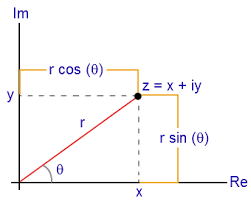
\includegraphics[width=0.5\linewidth]{Argand_plane}
	\caption{The Argand Plane.}
	\label{fig:argand}
\end{figure}
}

\begin{lemma}
	The Triangle Inequality is:
	$$\norm{z_1 + z_2} \leq \norm{z_1} + \norm{z_2}$$
	We can prove this using the argand representation. 
\end{lemma}

Properties of complex numbers:

\begin{itemize}
	\item Commutative
	\item Associative
	\item Distributive
	\item $z_1 -z_2 = z_1 + (-z_2)$.
	\item $z^n = r^n(\cos(n\theta) + i \sin(n\theta)$
	\item Complex Cojugate: $z^* = \bar{z} = x-iy = r(\cos\theta - i \sin\theta)$
	\item $z z^* = \norm{z}^2$
	\item Division 
\end{itemize}

\Def{Roots of Unity}{Given a complex number $z_0$ characterized by $r_0, \theta_0$, can we find a $z$ such that $z^n = z_0$? Well, clearly:
$$r^n = r_0$$
$$\cos(n\theta) + i \sin(n\theta) = \cos(\theta_0) + i \sin(n\theta_0)$$

This, $\norm{z} = r_0^{1/n}$, and $n\theta = \theta_0 + 2k\pi,\ k = 0, \pm 1, \pm 2...)$ There are only $n$ different solutions, meaning there are only $n$ roots. If we let $z_0 = 0$, we can find the roots of unity:

$$\text{roots of unity} = z = \cos(\frac{2k\pi}{n}) + i \sin(\frac{2k\pi}{n})$$
If we let $\omega = \cos(\frac{2\pi}{n}) + i \sin(\frac{2\pi}{n})$, then $\sum_{k=0}^{n-1} \omega^k = 0$

TODO: rebecca, this seems a bit wrong. See \href{https://en.wikipedia.org/wiki/Root_of_unity}{https://en.wikipedia.org/wiki/Root\_of\_unity} for a better explanation.

Essentially, geometrically, this means that the powers of $\omega$ sum to zero, as in Figure \ref{fig:3rdrootsofunity}.

\begin{figure}[H]
	\centering
	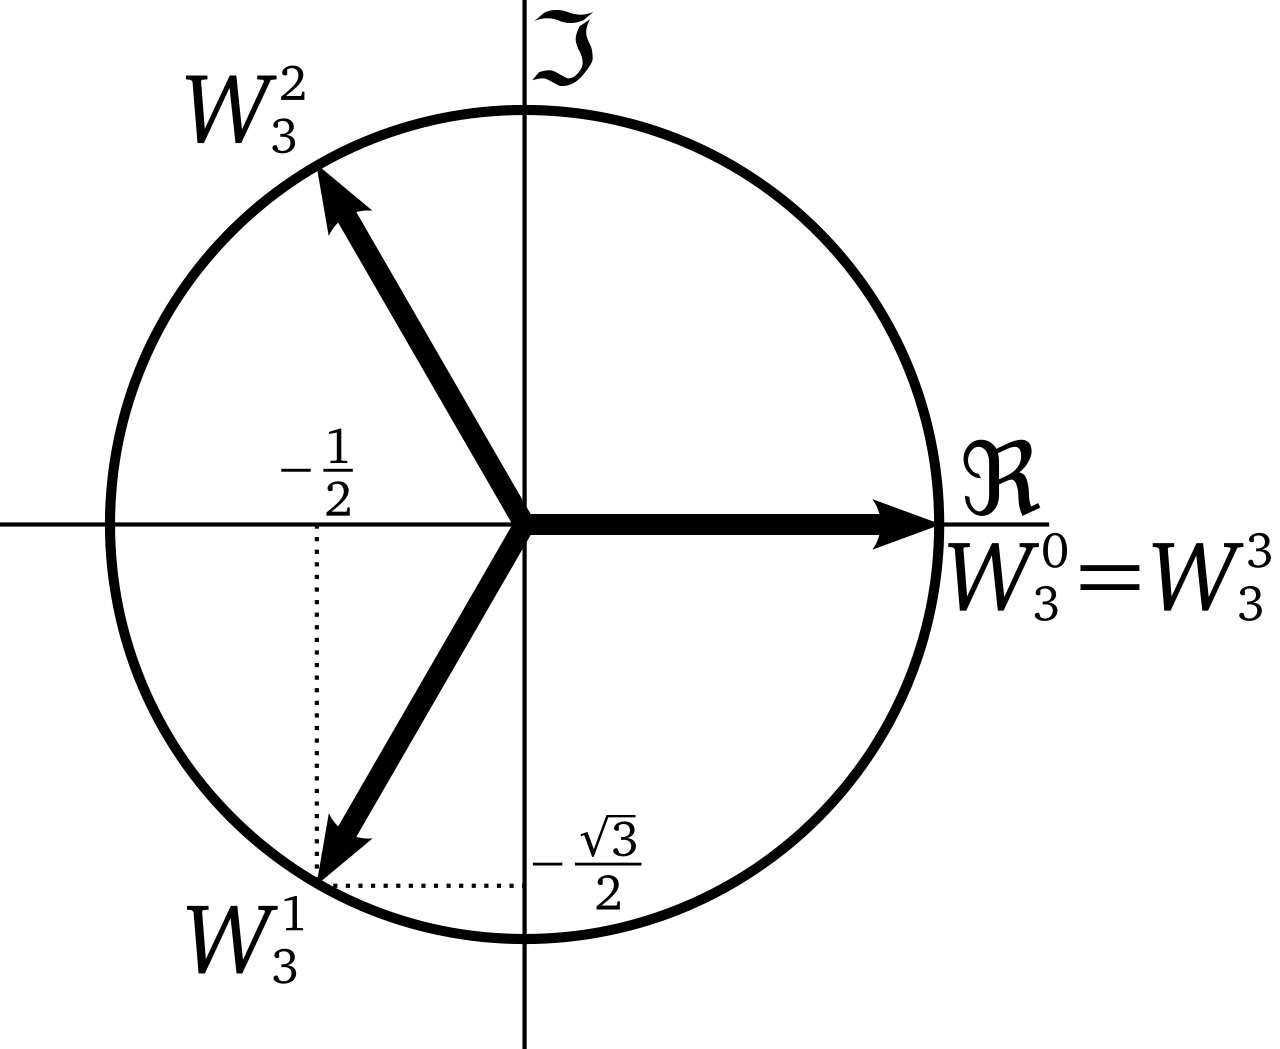
\includegraphics[width=0.5\linewidth]{3rd_roots_of_unity}
	\caption{The third roots of unity sum to one - as do nth roots of unity. \textit{Wikipedia.}}
	\label{fig:3rdrootsofunity}
\end{figure}

}

The complex numbers lack the notion of order, in the way the real numbers have order. In particular, the notion of $\infty$ is very different. For real numbers, we have $\pm \infty$, which serves as an upper and lower bound on $\R$. For complex numbers, we define a \textit{point at infinity}. The point at infinity is the limit of what happens as $r$ goes to infinity for $z=r e^{i\theta}$, While it may seem like this goes to a different point for different $\theta$, the point at infinity is in fact the same.

One way to imagine this is to consider the \textit{stereographic projection} (Figure \ref{fig:stereographic}):
\begin{figure}[H]
	\centering
	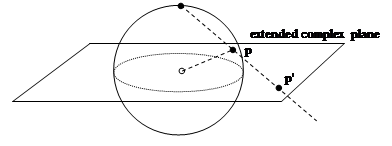
\includegraphics[width=0.5\linewidth]{stereographic_projection}
	\caption{The stereographic projection. We can see that as the point picked to move away from the point at infinity (the north pole), becomes horizontal. The intersection point on the sphere will gradually move closer to the point at the north pole, hence the north pole is the point at infinity. \textit{MathPages}.}
	\label{fig:stereographic}
\end{figure}








\end{document}